\documentclass[12pt,a4paper]{article}
\usepackage[utf8]{inputenc} % sempre salve seus arquivos como UTF8
\usepackage[T1]{fontenc}
\usepackage[english]{babel}

\usepackage[left=2.5cm,right=2cm,top=2cm,bottom=2.5cm]{geometry}
\usepackage{amsmath}
\usepackage{amsthm}
\usepackage{amsfonts}

\usepackage{graphicx}
\usepackage{algorithm}
\usepackage{color}
\usepackage[noend]{algpseudocode}
\usepackage{mathtools}
\usepackage{subfig}
\usepackage{diagbox}

% load times font
\usepackage{mathptmx}
\usepackage[scaled=.90]{helvet}
\usepackage{courier}

% comandos
\newcommand{\mdc}[1]{\mathrm{mdc}(#1)}

\DeclarePairedDelimiter\ceil{\lceil}{\rceil}
\DeclarePairedDelimiter\floor{\lfloor}{\rfloor}

% Foot without marker
\newcommand\blfootnote[1]{%
	\begingroup
	\renewcommand\thefootnote{}\footnote{#1}%
	\addtocounter{footnote}{-1}%
	\endgroup
}

\title{MO446 -- Introduction to Computer Vision  \\ Project 3}
\author{Breno Leite  \\ Guilherme Leite}
\date{05/10/2017}

\begin{document}

\maketitle
\blfootnote{\textit{\textbf{Important note:} The borders seen in the figures are not part of the image, they are figurative information about the starting and ending points of the image. Moreover, all the image scales in this report were changed in order to make the text more readable.}} \\

%% ---------------- Starts here --------------------------------

\textbf{\LARGE Input Images}\\

Throughout this project some images are used as input to test the algorithms. Figure \ref{fig:p1-1-0} was used as input for the pyramids exercises \textbf{2.1, 2.2, 2.3} and \textbf{3.1}, its dimensions are 400x300 and it is a colored image. \\

\begin{figure}[!h]
	\centering
	{%
		\setlength{\fboxsep}{1pt}%
		\setlength{\fboxrule}{1pt}%
		\fbox{
\includegraphics[scale=1]{input/p1-1-0}}%
	}%
	\caption{Input image for pyramids and Fourier transform exercises. (\textbf{p1-1-0})}
	\label{fig:p1-1-0}
\end{figure}

\begin{figure}[!h]
	\centering
	\subfloat[Orange to be blended (\textbf{p1-2-4-0})]{
		{
			\setlength{\fboxsep}{1pt}
			\setlength{\fboxrule}{1pt}
			\fbox{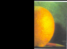
\includegraphics[scale=0.5]{input/p1-2-4-0}}
		}
                \label{fig:orangeBlend}
	}
	\quad
	\subfloat[Apple to be blended (\textbf{p1-2-4-1})]{
		{
			\setlength{\fboxsep}{1pt}
			\setlength{\fboxrule}{1pt}
			\fbox{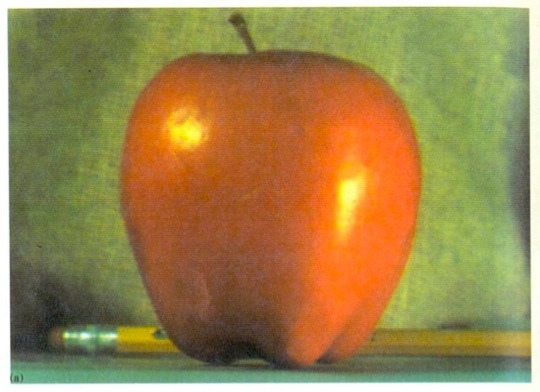
\includegraphics[scale=0.5]{input/p1-2-4-1}}
		}
	}
	\quad
	\subfloat[Mask for fruits blending (\textbf{p1-2-4-2})]{
		{
			\setlength{\fboxsep}{1pt}
			\setlength{\fboxrule}{1pt}
			\fbox{
\includegraphics[scale=0.25]{input/p1-2-4-2}}
		}
	}
	\caption{Initial images used on the blending experiments.}
	\label{fig:blending}
\end{figure}

\begin{table}[!h]
	\centering
	\begin{tabular}{|c|c|c|c|}
		\hline
		& \multicolumn{3}{c|}{\textbf{Time (seconds)}} \\ \hline
		\backslashbox{\textbf{Convolution}}{\textbf{Kernel Size}}    & \textbf{3x3}         & \textbf{7x7}          & \textbf{15x15}      \\ \hline
		\textbf{Implemented}  & 4.481      & 4.535      & 5.083     \\ \hline
		\textbf{OpenCV} & 0.001      & 0.004       & 0.010     \\ \hline
	\end{tabular}
	\caption{Comparison between our implementation and OpenCV convolution time.}
	\label{table:convolution-opencv}
\end{table}

\textbf{\LARGE Question 3 - Frequency Blending} \\

In this question, we will present some experiments developed using \emph{numpy} and \emph{OpenCV} functions in order to transform the image from spatial domain to frequency domain. The process will be divided into two different experiments for better readability. \\

On the first one (\textbf{3.1}), we will be modifying the phase and magnitude in order to see the impact on the image reconstructed on the Fourier transform. On the second experiment (\textbf{3.2}), we will be blending the two images used in Question \textbf{4.2} in order to compare frequency and spatial blending. \\

\textbf{3.1 )} Exploring Fourier Space \\

To explore the Fourier space, we implemented two different functions. The first one is responsible to transform an image into vectors of magnitude and phase, while the other is responsible to reconstruct the image from the magnitude and phase vectors. The Figure \ref{fig:mag-phase} shows the magnitude and phase obtained transforming the Figure \ref{fig:p1-1-0} to the frequency domain. \\

\end{document}
